\documentclass[12pt, a4paper]{article}
\setlength{\parindent}{0pt}
\usepackage{amsmath}
\usepackage{amsthm}
\usepackage{amssymb}
\usepackage[a4paper, portrait, margin=1in]{geometry}
\usepackage{graphicx}
\graphicspath{ {./} }

\renewcommand{\qedsymbol}{$\blacksquare$}

\newcommand{\R}{\mathbb{R}}
\newcommand{\Z}{\mathbb{Z}}
\newcommand{\displim}[1]{\displaystyle{\lim_{#1}\:}}
\newcommand{\zerolim}{\displim{x \to 0}}

% let's begin
\begin{document}
\textbf{(Q3)}

\textit{(a)}

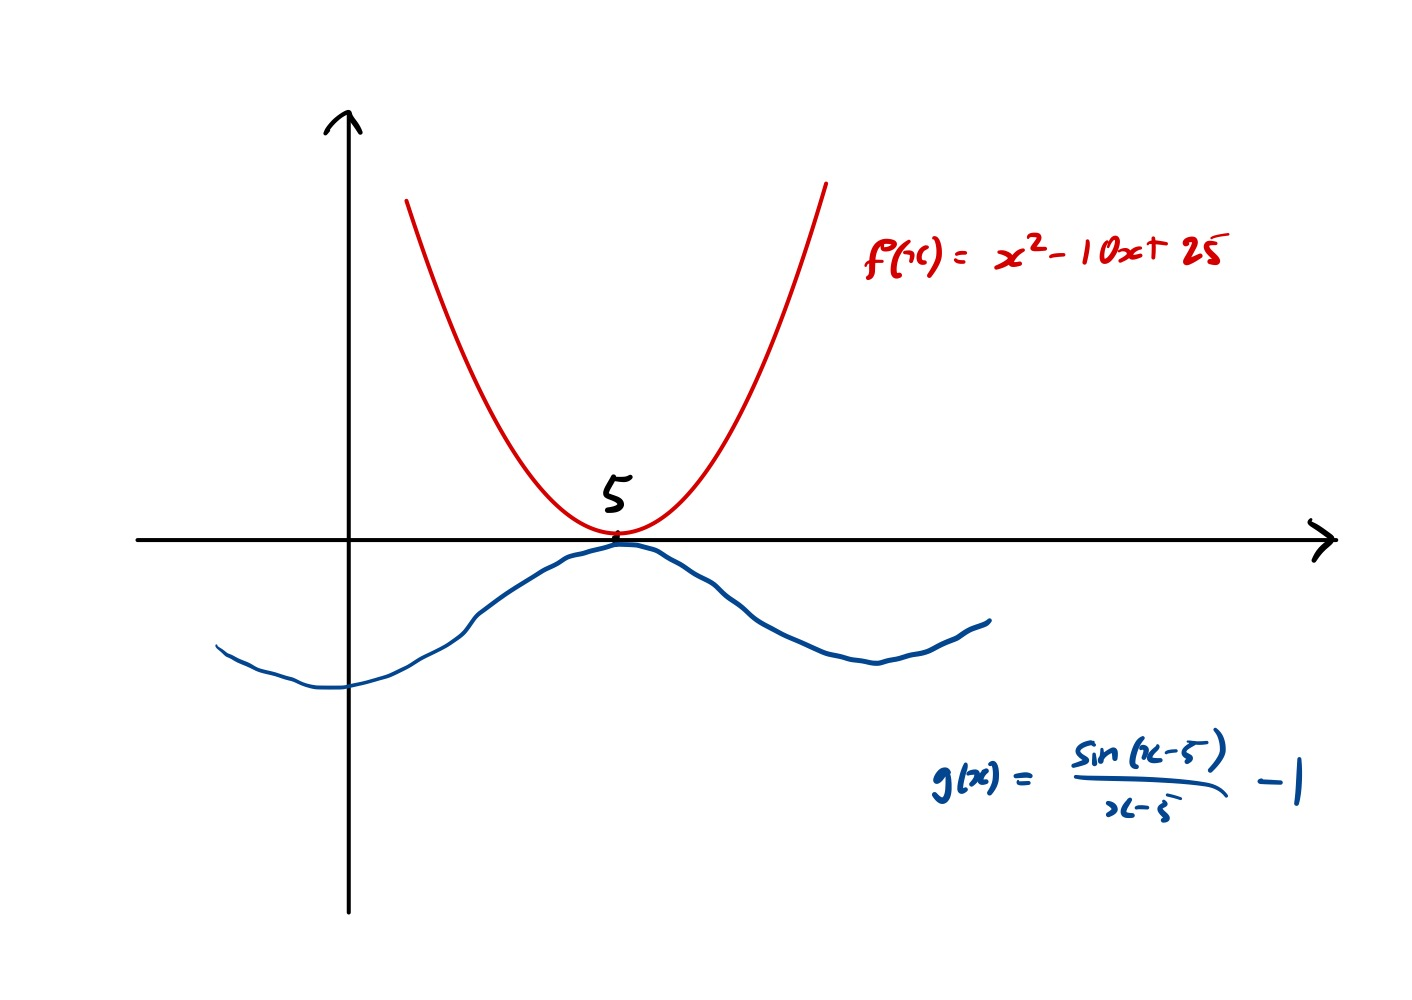
\includegraphics[width=\textwidth]{q3.jpg}

\newpage

\textit{(b)}

\begin{proof}
    In order to prove that $f(x)$ kisses $g(x)$ at $x = 0$, we need to prove that

    \begin{enumerate}
        \item $\forall x \neq a, \: f(x) > g(x)$ or $f(x) < g(x)$
        \item $\displim{x \to a} f(x) = \displim{x \to a} g(x)$.
    \end{enumerate}

    By limit laws,
    \[
        \displim{x \to 0} x^2 + 1 = \displim{x \to 0} x^2 + \displim{x \to 0} 1
        = 0 + 1 = 1
    \]

    By earlier proof, we also know:
    \[
        \displim{x \to 0} \frac{\sin x}{x} = 1 = \displim{x \to 0} x^2 + 1
    \]

    Which satisfies Condition 2.

    To prove Condition 1, we can use without proof that $\forall x \in \R\: |\sin x| \leq |x|$.
    Then $\forall x \neq 0$:

    \begin{align*}
        \frac{|\sin x|}{|x|} & \leq 1\\
        \implies \left|\frac{\sin x}{x}\right| & \leq 1\\
        \implies -1 \leq \frac{\sin x}{x} & \leq 1
    \end{align*}

    Considering $x^2$:

    \[
        x^2 \geq 0 \implies x^2 + 1 \geq 1
    \]

    Since $g(0) = 1$, $g(x) > 1 \text{ for all } x \neq 0$. Finally, for all $x \neq 0$,
    \[
        \frac{\sin x}{x} \leq 1 < x^2 + 1 \implies \frac{\sin x}{x} < x^2
    \]

    Which satisfies Condition 1.

    Since both conditions are satisfied, we have proven that $f(x)$ kisses $g(x)$ at $x = 0$, as required.
\end{proof}
\end{document}
